\documentclass[10pt]{beamer}

\usetheme[subsectionpage=progressbar]{metropolis}
\usepackage{appendixnumberbeamer}

\usepackage{booktabs}
\usepackage[scale=2]{ccicons}

\usepackage{pgfplots}
\usepgfplotslibrary{dateplot}

\usepackage{amsthm,amsmath,amsfonts}
\usepackage{dsfont}
\usepackage{xspace}
\usepackage{dsfont}
\usepackage{graphicx}
\newcommand{\themename}{\textbf{\textsc{metropolis}}\xspace}

\title{Boosting: Wisdom of the Crowd}
% \subtitle{Machine Learning in Produktion und Logistik}
\date{January 29, 2021}
\author{Christian Peters}
%\institute{TU Dortmund}
%\titlegraphic{\hfill\includegraphics[height=1.5cm]{logo.pdf}}

\begin{document}

\maketitle

%\begin{frame}{Contents}
%  \setbeamertemplate{section in toc}[sections numbered]
%  \tableofcontents
%\end{frame}

\begin{frame}{What you will know}

    \textbf{$\rightarrow$ The idea behind boosting}
    
    \vspace{0.8cm}
    
    \pause

    \textbf{$\rightarrow$ How to create a strong and efficient learning algorithm}

    \vspace{0.8cm}
    
    \pause

    \textbf{$\rightarrow$ What is AdaBoost and why is it so successful?}
\end{frame}

\section{Let's talk about training a model}

\begin{frame}{How to train a machine learning model}
    \textbf{What we have learned so far...}    
    \begin{itemize}
        \item We have to pick a hypothesis class $\mathcal{H}$ \pause
        \item $\mathcal{H}$ can't be too complex (VC dim needs to be finite) \pause
        \item We need enough training data (more than some threshold $m_\mathcal{H}$) \pause
        \item Then we use ERM to pick the best $h \in \mathcal{H}$ that minimizes the empirical error \pause
    \end{itemize}
    But there is one problem...
\end{frame}

\begin{frame}{The problem with ERM}
\setlength{\fboxrule}{2pt}
    \begin{center}
        \fbox{\huge \textbf{ERM can be hard.}}
    \end{center}

    \pause    
    
    \begin{itemize}
        \item Depending on $\mathcal{H}$, the optimization problem can become arbitrarily complex \pause
        \item e.g. implementing ERM for halfspaces in the non-separable case is computationally hard (chapter 9) \pause
        \item For many interesting classes, it is infeasible to implement ERM
        \begin{itemize}
            \item Solving the optimization problem takes forever
        \end{itemize}
    \end{itemize}

    \pause    
    
    \textbf{...so what can we do?}
\end{frame}

\begin{frame}{A first idea...}
    \textbf{Idea:} Use simpler hypothesis classes where ERM isn't hard.

    \pause    
    
    \begin{itemize}
        \item Problem: Simple classes can be too "weak" to estimate all relationships in the data
        \begin{itemize}
            \item[$\rightarrow$] Can lead to underfitting and poor performance
        \end{itemize} \pause
        \item Approximation error is high ($\rightarrow$ B/C tradeoff) \pause
        \item Still, these classes can be useful for us
        \begin{itemize}
            \item If the resulting hypothesis is at least better than random
        \end{itemize}
    \end{itemize}

    \pause    
    
    Let's call ERM on a simple class a \textbf{weak learner}. We will formally define it later...
\end{frame}

\begin{frame}{The idea behind boosting}
    \textbf{Why not combine many weak learners?}\\
    \textbf{Can this give us an efficient strong learner?}
    
    \pause    
    
    \begin{itemize}
        \item This theoretical question is the origin of boosting \pause
        \item It was first raised in 1988 by Kearns and Valiant~\cite{kv-lbffahf-88} \pause
        \item The first (practical) answer was given in 1995 by Freund and Schapire~\cite{FREUND1997119}
        \begin{itemize}
            \item[$\rightarrow$] It is YES!
        \end{itemize} \pause
        \item The result is \textbf{AdaBoost}, a widely popular and award winning algorithm
        \begin{itemize}
            \item We will take a look at this later...
        \end{itemize}
    \end{itemize}

    \pause    
    
    But first, let's get back to weak learning.
\end{frame}

\section{Weak Learnability}

Assuming that the realizable assumption~\cite[chapter 2]{SSBD14} holds, the generalization error
$L_{(\mathcal{D}, f)}(h)$ of a PAC learner with respect to a distribution $\mathcal{D}$ and a
labeling function $f$ can by the definition of PAC learning~\mbox{\cite[chapter 2]{SSBD14}} be reduced to an arbitrarily
small number (with confidence of $1-\delta$) by increasing the sample size of the training sequence $S$.
This, however, can be computationally infeasible in practical applications.

The concept of weak learnability aims to relax the requirement that the generalization error of a hypothesis must
become arbitrarily small the more the sample size is increased.
For weak learning, it is sufficient that the learning algorithm yields a hypothesis $h$, that performs only slightly
better than a random guess.
One can think of weak learning as applying a simple rule which isn't fully capable of modeling the data generating process,
but can still learn a little bit about the underlying problem so that it performs better than random.

Formally, the definition of a weak learner differs only slightly from the definition of PAC learning.
In the situation of a two-class classification problem, the definition of a weak learner, can be given as follows:

\begin{definition}{($\gamma$-weak-learner)}
\label{def:weak-learner}
An Algorithm $A$ is a $\gamma$-weak-learner for a hypothesis class $\mathcal{H}$ if for every $\delta \in (0, 1)$ there
exists a threshold $m_\mathcal{H}(\delta) \in \mathbb{N}$
such that for every distribution $\mathcal{D}$ over the instance space $\mathcal{X}$
and for every labeling function $f: \mathcal{X} \rightarrow \{\pm 1\}$ if running $A$ on $m \geq m_\mathcal{H}$ training
examples, it will yield a hypothesis $h$ such that with probability of at least $1-\delta$ the generalization error
$L_{(\mathcal{D}, f)}(h)$ is at most $\frac{1}{2} - \gamma$, provided that the realizable assumption holds.
\end{definition}

The parameter $\gamma$ in Definition \ref{def:weak-learner} tells us how well we can expect the weak learner to perform.
For example if a learning algorithm is a $1\%$-weak-learner for a class $\mathcal{H}$, then the generalization
error can at most be $49\%$ provided that first, the learner didn't fail
(which can happen with probability $\delta$ of drawing a bad sample from $\mathcal{D}$)
and second, the learner was run on at least $m_\mathcal{H}(\delta)$ training examples.

It still remains the question of how to obtain a weak learning algorithm.
We already saw that applying the ERM rule to complex hypothesis classes can be computationally hard.
But what if we choose a simple hypothesis class $B$ instead, where the ERM rule can be applied efficiently?
The following theorem states when we can obtain a weak learner for a hypothesis class $\mathcal{H}$ by
applying the ERM rule to a simpler class $B$.

\begin{theorem}
\label{theorem:erm-b}
Let $B$ and $\mathcal{H}$ be hypothesis classes and $\text{ERM}_B$ a learning algorithm that applies the ERM rule to $B$.
If for every distribution $\mathcal{D}$, for every $h \in \mathcal{H}$ and for every $\delta \in (0, 1)$
there exists a threshold $m_\mathcal{H}(\delta) \in \mathbb{N}$ such that for every sample
of $m \geq m_\mathcal{H}(\delta)$ i.i.d. examples generated by $\mathcal{D}$ and labeled by $h$, it holds that
$ERM_B$ returns a hypothesis $b \in B$ with $L_{(\mathcal{D}, h)}(b) \leq \frac{1}{2} - \gamma$,
then $ERM_B$ is a $\gamma$-weak-learner for $\mathcal{H}$.
\end{theorem}

\begin{proof}
	Theorem~\ref{theorem:erm-b} follows directly from Definition~\ref{def:weak-learner}.
\end{proof}

	
\section{AdaBoost}

\begin{frame}{AdaBoost - How it works}
    \begin{itemize} \pause
        \item AdaBoost invokes the weak learner $T$ times
            on the training data using different sample weights
            $(D_1^{(t)}, ..., D_m^{(t)}), \  t=1, ..., T$ \pause
        \item In every iteration $t$, the weak learner finds a hypothesis $h_t$ \pause
        \item Then, AdaBoost does a weighted majority vote:
    \end{itemize}
    \begin{equation*}
        h(x) = \text{sign}\left( \sum_{t=1}^T w_t h_t(x) \right)
    \end{equation*} \pause
    Let's look at this in more detail...
\end{frame}

\begin{frame}{One iteration of AdaBoost}
    \begin{enumerate} \pause
        \item Invoke the weak learner on the training data weighted by $D^{(t)}$
        \begin{itemize}
            \item In iteration $t=1$, we use equal weights $D_i^{(t)}=\frac{1}{m}$
        \end{itemize} \pause
        \item Compute a weight for the resulting hypothesis $h_t$ like this:
        \begin{equation*}
            w_t = \frac{1}{2} \text{log} \left( \frac{1}{\epsilon_t} - 1 \right)
        \end{equation*}
        \begin{itemize}
            \item $\epsilon_t$ is the (weighted) training error of $h_t$ \pause
        \end{itemize}
        \item Update the weights $D_i^{(t)}$ like this
        \begin{equation*}
            D_i^{(t+1)} = \frac{D_i^{(t)} \text{exp} \left( -w_t y_i h_t(\mathbf{x}_i) \right)}{
        \sum_{j=1}^m D_j^{(t)} \text{exp} \left( -w_t y_j h_t(\mathbf{x}_j) \right) }
        \end{equation*}
    \end{enumerate}
\end{frame}

\begin{frame}{A step by step example\footnote{Taken from the book \textit{Boosting: Foundations and Algorithms} written by Freund and Schapire~\cite{boosting}.
You can read it for free at \url{https://mitpress.mit.edu/books/boosting}}}
    \begin{figure}
        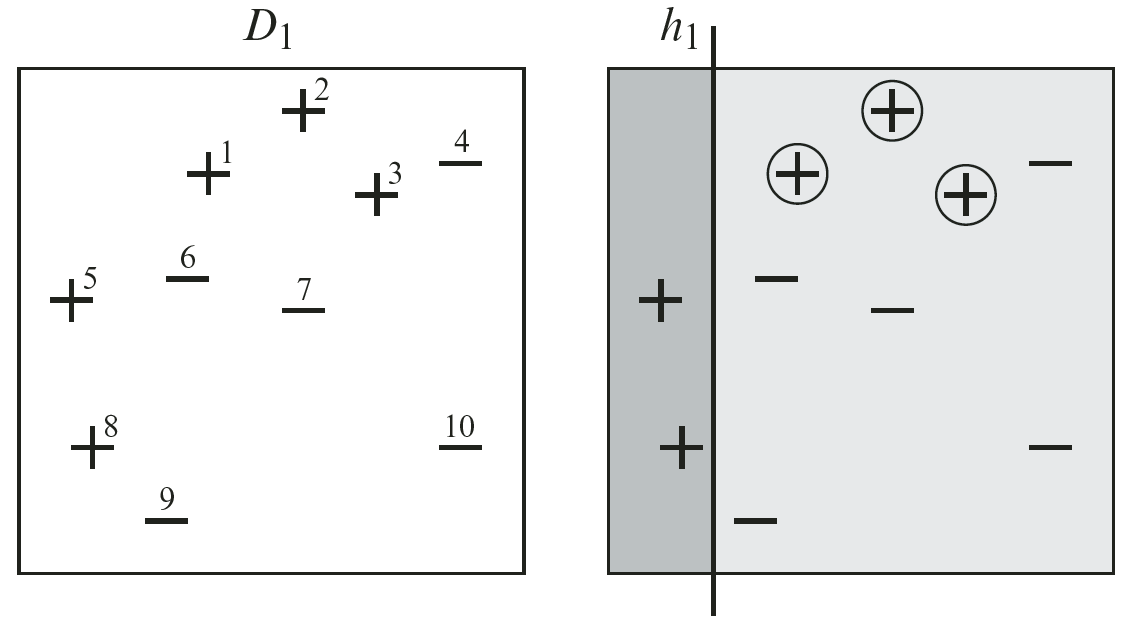
\includegraphics[width=\textwidth]{img/example_1}
    \end{figure}
\end{frame}

\begin{frame}{A step by step example}
    \begin{figure}
        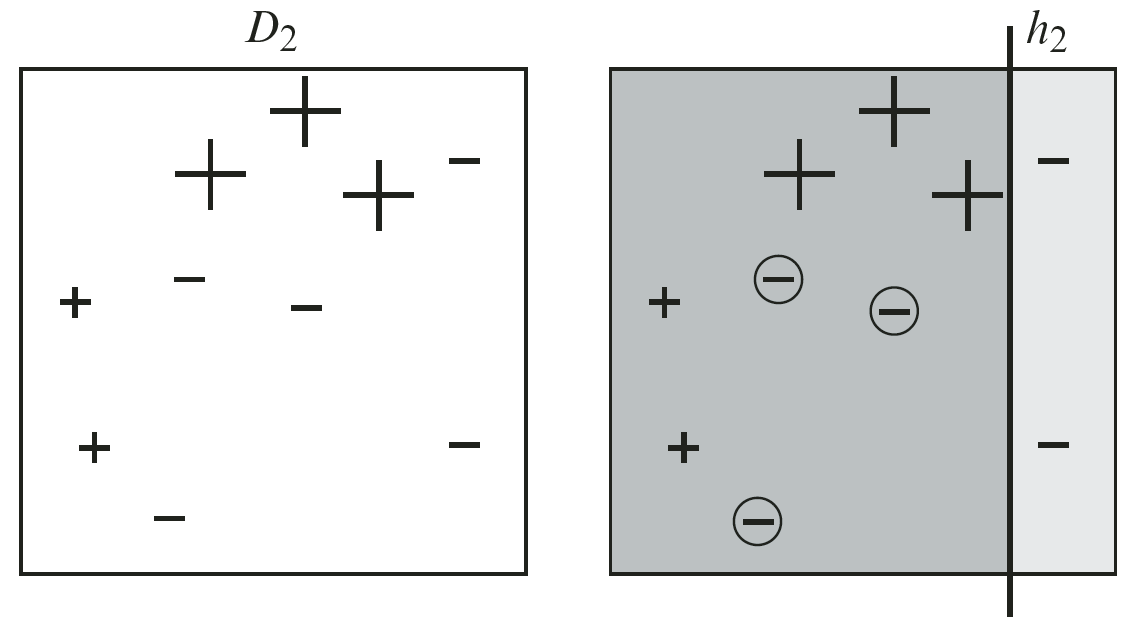
\includegraphics[width=\textwidth]{img/example_2}
    \end{figure}
\end{frame}

\begin{frame}{A step by step example}
    \begin{figure}
        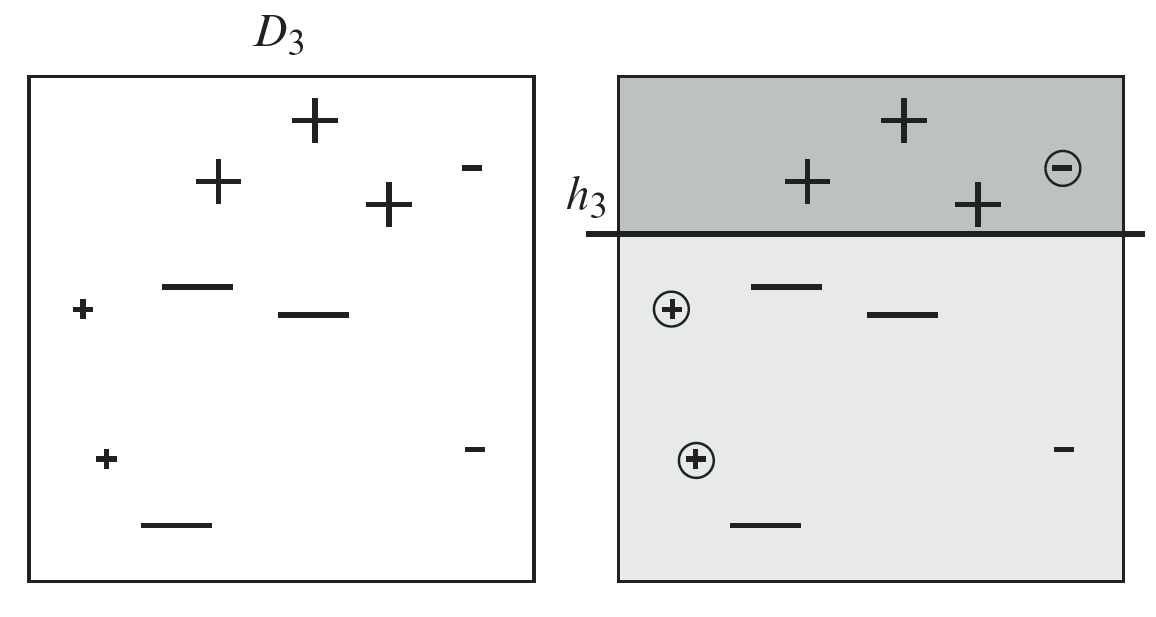
\includegraphics[width=\textwidth]{img/example_3}
    \end{figure}
\end{frame}

\begin{frame}{A step by step example}
    \begin{figure}
        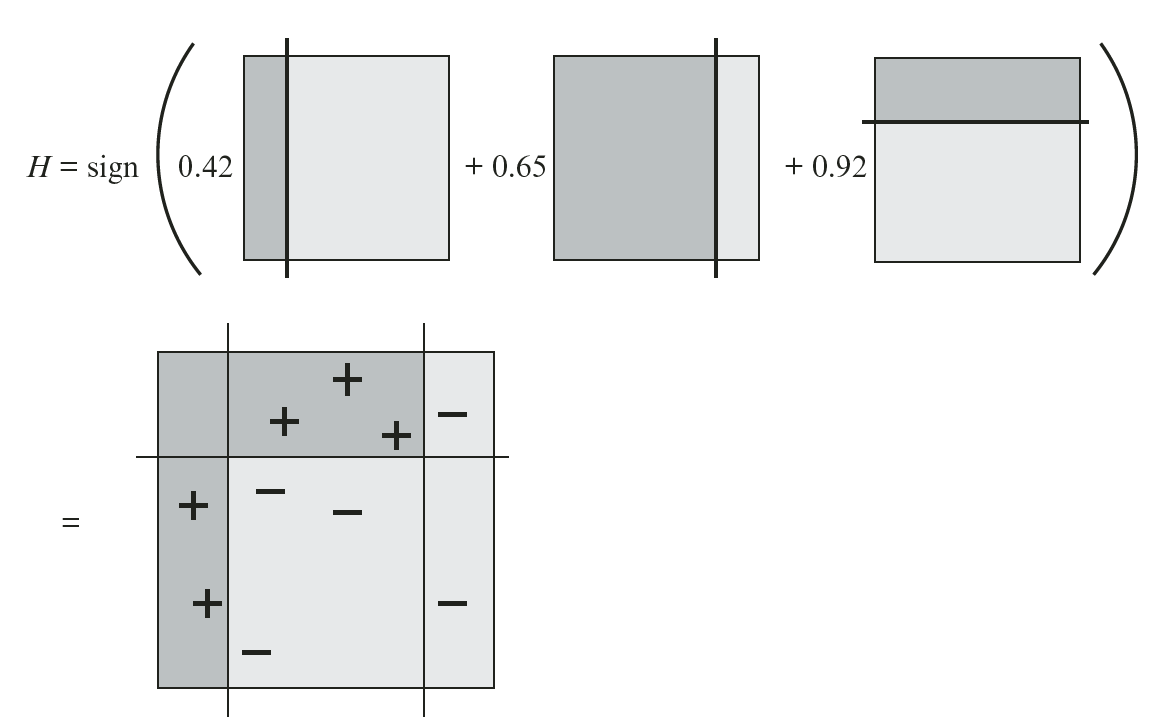
\includegraphics[width=\textwidth]{img/example_result}
    \end{figure}
\end{frame}

\begin{frame}{AdaBoost training error}
    \begin{itemize} \pause
        \item In the previous example, the training error was reduced to zero \pause
        \item What about the general case? \pause
        \begin{equation*}
            L_S(h) = \frac{1}{m} \sum_{i=1}^m \mathds{1}_{\left[ h(\mathbf{x}_i) \neq y_i \right]} \leq e^{-2 \gamma^2 T}
        \end{equation*} \pause
        \item The training error of AdaBoost decreases exponentially in $T$ \pause
    \end{itemize}
    \textbf{...but what about the out of sample error?}
\end{frame}

\section{Conclusion}
\label{conclusion}

In this article it was shown how a weak learning algorithm can be boosted into a strong PAC learner using the
AdaBoost algorithm.
The hypothesis class of decision stumps was identified to be efficiently learnable using an ERM algorithm, so
it followed that the AdaBoost algorithm is also efficient using decision stumps as the base learner.


\begin{frame}[standout]
  The End.
\end{frame}

\appendix

\begin{frame}[allowframebreaks]{References}

  \nocite{SSBD14, FREUND1997119, kv-lbffahf-88, boosting}

  \bibliography{bibliography}
  \bibliographystyle{abbrv}

\end{frame}

\end{document}
